\let\negmedspace\undefined
\let\negthickspace\undefined
\documentclass[a4,12pt,onecolumn]{IEEEtran}
%\documentclass[conference]{IEEEtran}
%\IEEEoverridecommandlockouts
% The preceding line is only needed to identify funding in the first footnote. If that is unneeded, please comment it out.
\usepackage{cite}
\usepackage{amsmath,amssymb,amsfonts,amsthm}
\usepackage{algorithmic}
\usepackage{graphicx}
\usepackage{textcomp}
\usepackage{xcolor}
\usepackage{txfonts}
\usepackage{listings}
\usepackage{enumitem}
\usepackage{mathtools}
\usepackage{gensymb}
\usepackage[breaklinks=true]{hyperref}
\usepackage{tkz-euclide} % loads  TikZ and tkz-base
\usepackage{listings}
\usepackage{empheq}
\usepackage{circuitikz}
%\usepackage{setspace}
%\usepackage{gensymb}
%\doublespacing
%\singlespacing

\usepackage{graphicx}
%\usepackage{amssymb}
%\usepackage{relsize}
%\usepackage[cmex10]{amsmath}
%\usepackage{amsthm}
%\interdisplaylinepenalty=2500
%\savesymbol{iint}
%\usepackage{txfonts}
%\restoresymbol{TXF}{iint}
%\usepackage{wasysym}
%\usepackage{amsthm}
%\usepackage{iithtlc}
%\usepackage{mathrsfs}
%\usepackage{txfonts}
%\usepackage{stfloats}
%\usepackage{bm}
%\usepackage{cite}
%\usepackage{cases}
%\usepackage{subfig}
%\usepackage{xtab}
%\usepackage{longtable}
%\usepackage{multirow}
%\usepackage{algorithm}
%\usepackage{algpseudocode}
%\usepackage{enumitem}
%\usepackage{mathtools}
%\usepackage{tikz}
%\usepackage{circuitikz}
%\usepackage{verbatim}
%\usepackage{tfrupee}
%\usepackage{stmaryrd}
%\usetkzobj{all}
%    \usepackage{color}                                            %%
\usepackage{array}                                            %%
%    \usepackage{longtable}                                        %%
%    \usepackage{calc}                                             %%
%    \usepackage{multirow}                                         %%
%    \usepackage{hhline}                                           %%
%    \usepackage{ifthen}                                           %%
  %optionally (for landscape tables embedded in another document): %%
%    \usepackage{lscape}     
%\usepackage{multicol}
%\usepackage{chngcntr}
%\usepackage{enumerate}

%\usepackage{wasysym}
%\newcounter{MYtempeqncnt}
\DeclareMathOperator*{\Res}{Res}
%\renewcommand{\baselinestretch}{2}
\renewcommand\thesection{\arabic{section}}
\renewcommand\thesubsection{\thesection.\arabic{subsection}}
\renewcommand\thesubsubsection{\thesubsection.\arabic{subsubsection}}

\renewcommand\thesectiondis{\arabic{section}}
\renewcommand\thesubsectiondis{\thesectiondis.\arabic{subsection}}
\renewcommand\thesubsubsectiondis{\thesubsectiondis.\arabic{subsubsection}}

% correct bad hyphenation here
\hyphenation{op-tical net-works semi-conduc-tor}
\def\inputGnumericTable{}                                 %%

\lstset{
%language=C,
frame=single, 
breaklines=true,
columns=fullflexible
}
%\lstset{
%language=tex,
%frame=single, 
%breaklines=true
%}

\begin{document}
%


\newtheorem{theorem}{Theorem}[section]
\newtheorem{problem}{Problem}
\newtheorem{proposition}{Proposition}[section]
\newtheorem{lemma}{Lemma}[section]
\newtheorem{corollary}[theorem]{Corollary}
\newtheorem{example}{Example}[section]
\newtheorem{definition}[problem]{Definition}
%\newtheorem{thm}{Theorem}[section] 
%\newtheorem{defn}[thm]{Definition}
%\newtheorem{algorithm}{Algorithm}[section]
%\newtheorem{cor}{Corollary}
\newcommand{\BEQA}{\begin{eqnarray}}
\newcommand{\EEQA}{\end{eqnarray}}
\newcommand{\define}{\stackrel{\triangle}{=}}

\bibliographystyle{IEEEtran}
%\bibliographystyle{ieeetr}


\providecommand{\mbf}{\mathbf}
\providecommand{\pr}[1]{\ensuremath{\Pr\left(#1\right)}}
\providecommand{\qfunc}[1]{\ensuremath{Q\left(#1\right)}}
\providecommand{\sbrak}[1]{\ensuremath{{}\left[#1\right]}}
\providecommand{\lsbrak}[1]{\ensuremath{{}\left[#1\right.}}
\providecommand{\rsbrak}[1]{\ensuremath{{}\left.#1\right]}}
\providecommand{\brak}[1]{\ensuremath{\left(#1\right)}}
\providecommand{\lbrak}[1]{\ensuremath{\left(#1\right.}}
\providecommand{\rbrak}[1]{\ensuremath{\left.#1\right)}}
\providecommand{\cbrak}[1]{\ensuremath{\left\{#1\right\}}}
\providecommand{\lcbrak}[1]{\ensuremath{\left\{#1\right.}}
\providecommand{\rcbrak}[1]{\ensuremath{\left.#1\right\}}}
\theoremstyle{remark}
\newtheorem{rem}{Remark}
\newcommand{\sgn}{\mathop{\mathrm{sgn}}}
%\providecommand{\abs}[1]{\left\vert#1\right\vert}
\providecommand{\res}[1]{\Res\displaylimits_{#1}} 
%\providecommand{\norm}[1]{\left\lVert#1\right\rVert}
%\providecommand{\norm}[1]{\lVert#1\rVert}
\providecommand{\mtx}[1]{\mathbf{#1}}
%\providecommand{\mean}[1]{E\left[ #1 \right]}
\providecommand{\fourier}{\overset{\mathcal{F}}{ \rightleftharpoons}}
%\providecommand{\hilbert}{\overset{\mathcal{H}}{ \rightleftharpoons}}
\providecommand{\system}{\overset{\mathcal{H}}{ \longleftrightarrow}}
	%\newcommand{\solution}[2]{\textbf{Solution:}{#1}}
\newcommand{\solution}{\noindent \textbf{Solution: }}
\newcommand{\cosec}{\,\text{cosec}\,}
\providecommand{\dec}[2]{\ensuremath{\overset{#1}{\underset{#2}{\gtrless}}}}
\newcommand{\myvec}[1]{\ensuremath{\begin{pmatrix}#1\end{pmatrix}}}
\newcommand{\mydet}[1]{\ensuremath{\begin{vmatrix}#1\end{vmatrix}}}
%\numberwithin{equation}{section}
%\numberwithin{equation}{subsection}
%\numberwithin{problem}{section}
%\numberwithin{definition}{section}
%\makeatletter
%\@addtoreset{figure}{problem}
%\makeatother

%\let\StandardTheFigure\thefigure
\let\vec\mathbf

\title{
\Huge\textbf{Analog Assignment}\\
\Huge\textbf{EE1205} Signals and Systems\\
}
\large\author{Nimal Sreekumar\\EE23BTECH11044}

% make the title area
\maketitle


%\tableofcontents

\bigskip

\renewcommand{\thefigure}{\theenumi}
\renewcommand{\thetable}{\theenumi}
%\renewcommand{\theequation}{\theenumi}


\textbf{Question 12.7.18:}
A circuit containing a 80mH inductor and a 60$\mu$F capacitor in series is connected to a 230V, 50Hz supply. The resistance of the circuit is negligible.\\
\begin{enumerate}
\item Obtain the current amplitude and rms value.
\item Obtain the rms value of potential drops across each element.
\item What is the average power transferred to the inductor ?
\item What is the average power transferred to the capacitor ?
\item What is the total average power absorbed by the circuit ? 
\end{enumerate}
\brak{\text{'Average' implies 'averaged over one cycle'.}}\\
\vspace{0.5mm}
\solution\\
\input{ncert12_7_18.tex}
\begin{table}[htbp]
\centering
\renewcommand\thetable{1}
\begin{tabular}{|c|c|m{3cm}|}
    \hline
    \textbf{Variable} & \textbf{values} & \textbf{Description} \\
    \hline
    $X_L$ & $\omega L = 8\pi$ & inductive reactance\\
    \hline
    $ X_C $ & $\frac{1}{\omega C} = \frac{1000}{6\pi}$& capacitive reactance\\
    \hline
    $I_0$ & ? & peak current\\
    \hline
    $I_{rms}$ & $I_{rms}=\frac{I_0}{\sqrt 2}$ & rms current\\
    \hline
   $V_{0}$ & $230\sqrt 2 V$ & peak voltage\\
    \hline
     $V_{rms}$ & $230 V$ & rms voltage\\
    \hline
     $Z$ & $?$ & impedence\\
    \hline
     $\omega$ & $100\pi$ & angular frequency\\
    \hline
\end{tabular}
\caption{Input Parameters}
\label{tab:12.7.18}
\end{table}

\begin{enumerate}
    \item 
    \begin{align}
    H\brak{s} &= sL + \frac{1}{sC}\\
    H\brak{j\omega} &= j\omega L + \frac{1}{j\omega C}\\
    |H\brak{j\omega}| &=\sqrt{(X_C - X_L)^2} \\
    &= \frac{1}{\omega C} - \omega L \\
    &= \frac{1000}{6\pi}- 8\pi \\
    &= 27.958\Omega   
    \end{align}
    Then,
    \begin{align}
        I_0 &= \frac{V_0}{|H\brak{j\omega}|} \\
        &= 11.63\, \text{A} \\
        I_{rms} &= \frac{I_0}{\sqrt{2}} = 8.22\, \text{A}
    \end{align}
    
    \item Voltage across the inductor:
    \begin{align}
        |V_L\brak{s}| &= |I_{rms} \times X_L| \\
        &= 206.48V
    \end{align}
    Voltage across the capacitor:
    \begin{align}
       |V_C\brak{s}| &= |I_{rms} \times X_C| \\
        &= 436.3V
    \end{align}

    \item Instantaneous power,
    \begin{align}
        P &= VI \\
        P &= V_0sin\brak{\omega t} I_0 sin\brak{\omega t - \phi}
    \end{align}
    Average power,
    \begin{align}
    P_{avg} &= \frac{W}{T} \implies dW = Pdt \\
    W &= V_0 I_0 \int_{0}^{T} sin\brak{\omega t} sin\brak{\omega t - \phi} dt \\
     W &= V_0 I_0 \int_{0}^{T} sin\brak{\omega t}\brak{sin\brak{\omega t}cos\brak{\phi}} - cos\brak{\omega t}sin\brak{\omega t} dt\\
       W &= V_0 I_0 \int_{0}^{T} \brak{sin\brak{\omega t}}^2 cos\brak{\phi}dt - V_0 I_0\int_{0}^{T}sin\brak{\omega t}cos\brak{\omega t}sin\brak{\phi} dt\\
        W &= V_0 I_0 \int_{0}^{T} \frac{1-cos{2 \omega t}}{2} cos\brak{\phi}dt - V_0 I_0\int_{0}^{T}sin\brak{2 \omega t}sin\brak{\phi}dt
    \end{align}
After solving,
    \begin{align}
        W &= \frac{1}{2} V_0 I_0 T cos{\phi} \\
        P_{avg} &=\frac{1}{2} V_0 I_0 cos{\phi}
    \end{align}
    Converting to rms terms,
    \begin{align}
      P_{avg} &= V_{rms} I_{rms} cos{\phi} \\
      tan\brak{\phi} &= \frac{\frac{1}{\omega C} -\omega L}{R} = \infty\\
      \phi &= \frac{\pi}{2} 
    \end{align}

 voltage across the capacitor leads the current by $90^\circ$,
    \begin{align}
        \text{Average power across inductor} (P_L) = 0
    \end{align}

    \item 
    Similarly, since voltage across the capacitor lags the current by $90^\circ$,
    \begin{align}
        \text{Average power across capacitor} (P_C) = 0
    \end{align}

    \item 
    \begin{align}
        \text{Total average power} &= P_L + P_C \\
        &= 0
    \end{align}
\end{enumerate}

\begin{figure}[ht]
\centering
   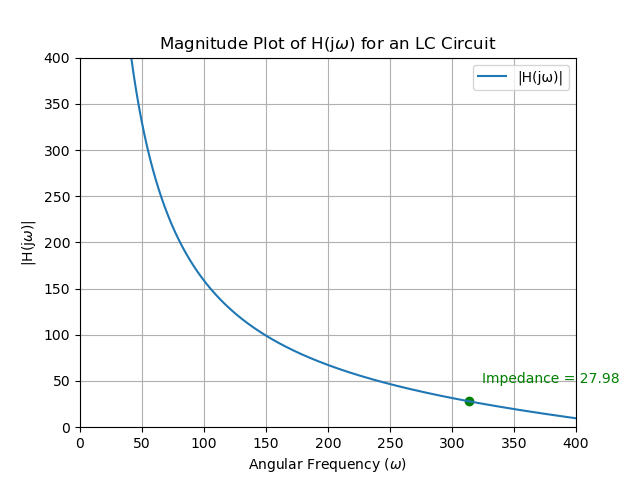
\includegraphics[width=1\linewidth]{12_7_18plot.png}
   \label{fig:12_7_18}
 \end{figure}

\end{document}
